% -*- coding: utf-8 -*-
\newpage

One of the simplest molecular properties that can be partitioned into atomic
contributions is the atomic charge. Following the definition of atomic basins,
the charge associated with a given atom is obtained as the difference between
the nuclear charge and the number of electrons within its basin:
%
\begin{align}
  q(\Omega) = Z_\Omega - \int_{\Omega} \rho(\mathbf{r}) \dd\tau.
  \label{q_qtaim}
\end{align}

While the decomposition of some properties such as charge is relatively
straightforward, the partitioning of other quantities requires more
elaborate treatments. In the following sections, we examine how QTAIM enables
the decomposition of the molecular dipole moment and polarisability into
well-defined atomic contributions.

\subsection{Dipole Moment}

The electric dipole moment is a vector quantity that characterises the spatial
distribution of positive and negative charge within a molecular system.
Classically, it is defined as the product of a point charge and its
displacement vector, $\mathbf{p} = q \mathbf{d}$. In molecular systems, however, the
total dipole moment $\boldsymbol{\mu}$ arises from the combined contributions of all
nuclei and electrons. It is conventionally expressed as the sum of nuclear
($\boldsymbol{\mu}_c$) and electronic ($\boldsymbol{\mu}_p$) components:
$\boldsymbol{\mu} = \boldsymbol{\mu}_c + \boldsymbol{\mu}_p$.

The nuclear contribution is straightforward to evaluate, involving the sum of
the nuclear charges $Z_A$ weighted by their position vectors $\mathbf{R}_A$
(Equation~\ref{mu_nuc}). The electronic component, by contrast, involves
integrating the position operator $\hat{r}$ weighted by the electron density
$\rho(\mathbf{r})$ over all space (Equation~\ref{mu_ele}):
%
\begin{align}
  \boldsymbol{\mu}_c &= \sum_A Z_A \mathbf{R}_A,
    \label{mu_nuc} \\
  \boldsymbol{\mu}_p &= - \int_{\rreal[3]} \mathbf{r} \rho(\mathbf{r}) \dd\tau.
    \label{mu_ele}
\end{align}

\pagebreak
In practical computational implementations, the electronic contribution to the
dipole moment is typically expressed in terms of the one-electron density
matrix $P_{\mu\nu}$ and the atomic orbital basis functions $\mu$ and $\nu$:
%
\begin{align}
  \boldsymbol{\mu}_p = -\sum_{\mu\nu} P_{\mu\nu} \matrixel{\mu}{\mathbf{r}}{\nu}.
\end{align}


{\small
\follow{Dipole moment decomposition}{
  Within QTAIM, both the nuclear and electronic components can be further
  decomposed into contributions from the atomic basins $\Omega_\alpha$.  This
  results in an atom-based decomposition of the total molecular dipole moment:
  \begin{align}
    \boldsymbol{\mu} &= \boldsymbol{\mu}_c + \boldsymbol{\mu}_p \nonumber \\
      &=\sum_\alpha Z_\alpha \mathbf{R}_\alpha
        - \sum_\alpha\int_{\Omega_\alpha} \mathbf{r}\rho(\mathbf{r})\dd\tau \nonumber \\
      &= \sum_\alpha \left(Z_\alpha \mathbf{R}_\alpha -
        \int_{\Omega_\alpha} (\mathbf{r}-\mathbf{R}_\alpha)\rho(\mathbf{r})\dd\tau 
        -\int_{\Omega_\alpha} \mathbf{R}_\alpha\rho(\mathbf{r})\dd\tau\right) \nonumber \\
      &= \sum_\alpha \left(q_\alpha \mathbf{R}_\alpha
        - \int_{\Omega_\alpha} (\mathbf{r}-\mathbf{R}_\alpha)\rho(\mathbf{r})\dd\tau \right) 
  \end{align}
}}

Although the nuclear contribution to the dipole moment is
origin-dependent, QTAIM allows a reformulation based on
\glspl{BCP} that offers additional physical insight~\cite{Keith}:
%
\begin{align}
  \boldsymbol{\mu}_c (\Omega)= \sum_{\Lambda}[\mathbf{R}_\Omega-\mathbf{R}_\mathrm{BCP}(\Omega|\Lambda)]Q(\Omega|\Lambda),
  \label{atomic_dipole}
\end{align}

\noindent where, $\mathbf{R}_\Omega$ is the centroid of atomic basin $\Omega$, 
$\mathbf{R}_\mathrm{BCP}(\Omega|\Lambda)$ denotes the position vector of the BCP between atoms
$\Omega$ and $\Lambda$, and $Q(\Omega|\Lambda)$ is the bond charge shared
between the two atoms. The computation of these bond charges is non-trivial,
particularly in systems with complex bonding topologies. Their values are obtained
by solving a linear system derived from charge conservation and symmetry
constraints:
%
\begin{align}
  q(\Omega) &= \sum_{\Lambda} Q(\Omega|\Lambda) \label{allbond}, \\
  Q(\Omega|\Lambda) &= -Q(\Lambda|\Omega) \label{symmetry}, \\
  0 &= \sum_{\Omega} Q(\Omega|\Omega+1) \label{ring},
\end{align}

\noindent where, $q(\Omega)$ denotes the QTAIM atomic charge, as defined in
Equation~\ref{q_qtaim}. Equation~\ref{ring} follows directly from the
combination of Equations~\ref{allbond} and~\ref{symmetry}. Solving this system
requires prior knowledge of both the QTAIM atomic charges and the full bonding
topology of the molecule, including the presence of ring structures.

\begin{wrapfigure}[5]{r}{0.3\textwidth}
  \centering
  \vspace{-2.5em}%
  \begingroup
\setmainfont{DejaVu Sans}

\resizebox{\linewidth}{!}{
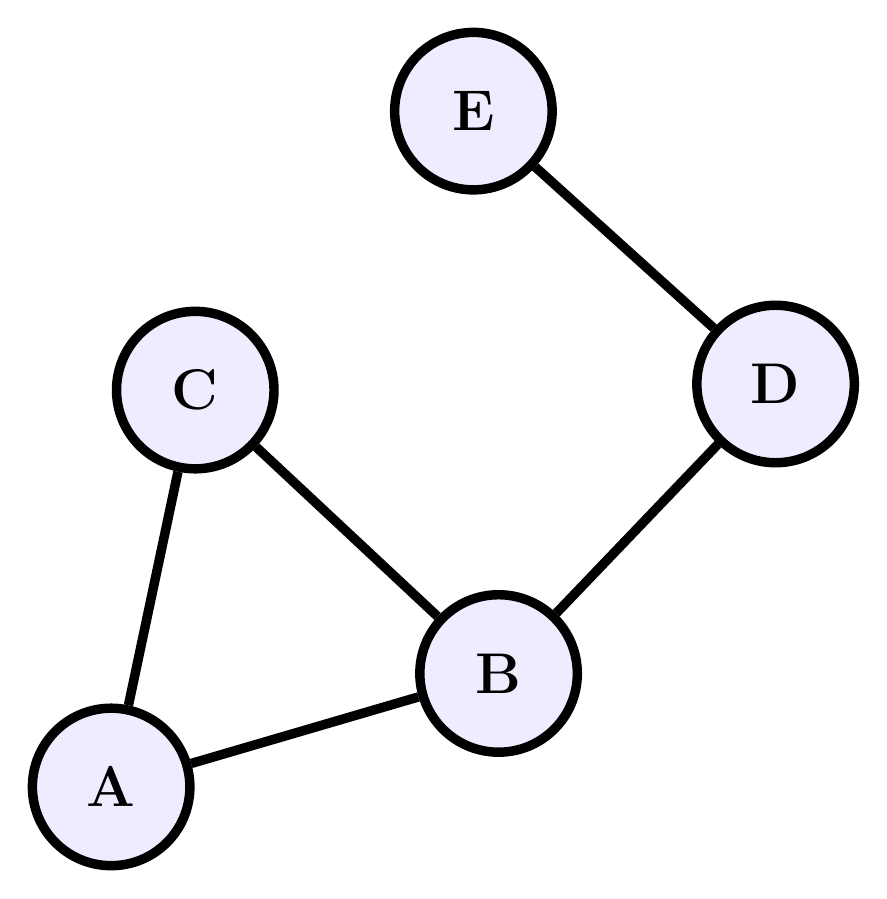
\begin{tikzpicture}

  \tikzset{
    mynode/.style={
      circle,
      draw=black,
      fill=blue!7,
      line width=1.2mm,
      minimum size=20mm,
      font=\bfseries\fontsize{20}{20}\selectfont,
      text centered
    }
  }

  \node[mynode] (A) at (110.1pt, 106.1pt) {A};
  \node[mynode] (B) at (250.1pt, 147.1pt) {B};
  \node[mynode] (C) at (140.5pt, 249.5pt) {C};
  \node[mynode] (D) at (350.2pt, 251.7pt) {D};
  \node[mynode] (E) at (241pt, 350.3pt) {E};

  \draw[black, line width=1.2mm] (A) -- (B);
  \draw[black, line width=1.2mm] (A) -- (C);
  \draw[black, line width=1.2mm] (B) -- (C);
  \draw[black, line width=1.2mm] (B) -- (D);
  \draw[black, line width=1.2mm] (D) -- (E);

\end{tikzpicture}
}
\endgroup


  % \includegraphics[width=0.3\textwidth]{img/abcde_charges}
  \caption{Graph of a system with 5 atoms and 1 ring.}
  \label{example_charges}
\end{wrapfigure}

% \vspace{1em}%
The minimal linear system required to solve the bond-charge decomposition
problem involves $N_{\text{BCP}}$ variables and a total of $N_{\text{atoms}} +
N_{\text{RCP}}$ equations. A hypothetical topology is shown in
Figure~\ref{example_charges}, and its corresponding matrix representation is
given in Equation~\ref{linear_system}.

\vspace{1em}%
\begin{align}
  \overbrace{
    \begin{pmatrix}
      \phantom{-}1 &  \phantom{-}1 &  \phantom{-}0 &  \phantom{-}0 &  \phantom{-}0 \\
     -1 &  \phantom{-}0 &  \phantom{-}1 &  \phantom{-}1 &  \phantom{-}0 \\
     \phantom{-}0 & -1 & -1 &  \phantom{-}0 & \phantom{-}0 \\
      \phantom{-}0 &  \phantom{-}0 &  \phantom{-}0 & -1 &  \phantom{-}1 \\
      \phantom{-}0 &  \phantom{-}0 &  \phantom{-}0 &  \phantom{-}0 &  -1 \\
      \phantom{-}1 & -1 &  \phantom{-}1 &  \phantom{-}0 &  \phantom{-}0
    \end{pmatrix}
  }^{\text{NBCP}}
    \begin{pmatrix}
      Q(A|B) \\
      Q(A|C) \\
      Q(B|C) \\
      Q(B|D) \\
      Q(D|E)
      \end{pmatrix}
    =
    \begin{pmatrix}
      q(A) \\
      q(B) \\
      q(C) \\
      q(D) \\
      q(E) \\
      0
    \end{pmatrix}
    \begin{array}{l}
      \left.\begin{array}{@{}c@{}}
      \\
      \\
      \\
      \\
      \\
    \end{array}\right\}\ \text{N atoms} \\[1ex]
      \left.\begin{array}{@{}c@{}}
      \\
    \end{array}\right\}\ \text{NRCP}
  \end{array}
  \label{linear_system}
\end{align}

\subsection{Polarisability}

The molecular polarisability describes the response of a molecule's dipole moment
to an external electric field $\mathbf{F}$. It plays a central role in determining
macroscopic properties such as the dielectric constant of bulk media, as captured
by the Clausius-Mossotti relation~\cite{landau2013electrodynamics}. At the
molecular level, the polarisability is a symmetric
$3 \times 3$ tensor, defined as:
%
\keq{Polarisability tensor}{
  \begin{align}
    \underline{\underline{\alpha}} =
      \left( \pdv{\mu_i}{F_j} \right)_{F=0}
  \end{align}
}

\newpage
A scalar measure of the polarisability, independent of the coordinate
system, is given by the isotropic mean polarisability. Owing to the invariance
of the trace under orthogonal transformations:
%
\begin{align}
  \bar{\alpha} = \sfrac{1}{3}\, \text{Trace}(\underline{\underline{\alpha}}).
\end{align}

% naïve 

Polarisabilities can be computed either analytically (\eg, via sum-over-states
methods) or numerically. The numerical approach relies on a finite-difference
approximation of the derivative, in which dipole moments are evaluated under
small applied electric fields~\cite{DosSantos2015}.

\begin{wrapfigure}{r}{0.48\textwidth}
  \centering
  % Cube with E field applied in x and z directions
% Dependecies in the file style/tikz_field.tex

\begin{tikzpicture}[
  font = \tiny \boldmath,
  tdplot_main_coords,
  anchor=center,
  inner sep = 3pt,
  axis/.style={->,blue,line width=0.8pt},
  cube/.style={draw=b,line width=0.6pt,line join=round,line cap=round},
  scale=1.8,
  face/.style={cube,line width=0.6pt,draw=b},
  filled face/.style={face,fill=w,opacity=0.8},
  arrow style/.style={-stealth,line width=0.5pt},
  ]

  \def\gridrange{1.7,2.07,2.43,2.8}
  \def\zrange{0.2,0.57,0.93,1.3}

  % Axes
  \begin{scope}[shift={(-0.2,0,-1.5)}, scale=0.8]
    \draw[-stealth] (0,0,0) -- (0.5,0,0) node[scale=0.9, anchor=east] {x};
    \draw[-stealth] (0,0,0) -- (0,0.7,0) node[scale=0.9, anchor=north east] {y};
    \draw[-stealth] (0,0,0) -- (0,0,0.4) node[scale=0.9, anchor=south] {z};
  \end{scope}

  % Blue plane
  \draw[cube, fill=sky, opacity=.5] (1.5,1.5,-0.3) -- (3,1.5,-0.3) -- (3,3,-0.3) -- (1.5,3,-0.3) -- cycle;
  \draw[cube,thick,draw=sky] (1.5,1.5,-0.3) -- (3,1.5,-0.3) -- (3,3,-0.3) -- (1.5,3,-0.3) -- cycle;

  % Pink plane
  \draw[cube, fill=pink!90, opacity=.4] (1.1,1.5,0) -- (1.1,3,0) -- (1.1,3,1.5) -- (1.1,1.5,1.5) -- cycle;
  \draw[cube,thick,draw=pink] (1.1,1.5,0) -- (1.1,3,0) -- (1.1,3,1.5) -- (1.1,1.5,1.5) -- cycle;

  % Cube Faces
  \foreach \face in {
    {(1.5,1.5,0) -- (3,1.5,0) -- (3,1.5,1.5) -- (1.5,1.5,1.5) -- cycle},
    {(1.5,3,0) -- (3,3,0) -- (3,1.5,0) -- (1.5,1.5,0) -- cycle},
    {(1.5,1.5,0) -- (1.5,1.5,1.5) -- (1.5,3,1.5) -- (1.5,3,0) --cycle}
  } {
    \draw[cube,thick, fill=b!20] \face;
  }

  % z component of E [Arrows]
  \foreach \x in \gridrange {
    \foreach \y in \gridrange {
      \pgfmathsetmacro{\op}{min(1, 0.7*((\y-1.4)/1.5 + (\x+0.5)/1.5)/2)}
      \draw[arrow style, sky, opacity=\op]
      (\x,\y,-0.7) -- (\x,\y,2);
    }
  }

  % Cube edge [Above the blue arrows but below the pink arrows]
  \foreach \face in {
    {(3,1.5,0) -- (3,3,0) -- (3,3,1.5) -- (3,1.5,1.5) -- cycle},
  } {
    \draw[face, thick] \face;
  }

  % x component of E [Arrows]
  \foreach \y in \gridrange {
    \foreach \z in \zrange {
      \pgfmathsetmacro{\op}{min(1, 1.4*((\y-1.4)/1.5 + (\z+0.5)/1.5)/2)}
      \draw[arrow style, pink, opacity=\op]
        (0.6,\y,\z) -- (3.6,\y,\z);
    }
  }

  % Cube edges [Above everything]
  \foreach \face in {
    {(1.5,3,0) -- (3,3,0) -- (3,3,1.5) -- (1.5,3,1.5)},
    {(1.5,1.5,1.5) -- (1.5,3,1.5) -- (3,3,1.5) -- (3,1.5,1.5)},
    {(1.5,3,0) -- (1.5,3,1.5)}
  } {
    \draw[face, thick] \face;
  }

  % Labels
  \begin{scope}[canvas is xz plane at y=2.25]
    \node[scale=1.1, text=pink, inner sep=2pt, xscale=-1, transform shape] at (0.1,0.6) {$F_x$};
  \end{scope}

  \begin{scope}[canvas is xz plane at y=3]
    \node[scale=1.1, text=sky, inner sep=2pt, xscale=-1, transform shape] at (2.27,-0.5) {$F_z$};
  \end{scope}

\end{tikzpicture}


  \caption{System in a box, subjected to an external electric field in $x$-axis
           and $z$-axis.} 
  \label{efield_cube}
\end{wrapfigure}

\vspace{1em}%
Figure~\ref{efield_cube} illustrates a molecular system placed in a simulation
box and subjected to external electric fields applied along two Cartesian
directions. A common approach to computing the polarisability involves
comparing the dipole moment of the system in the presence of a small electric
field with that of the unperturbed system. However, this method can lead to
reduced numerical accuracy, as it mixes contributions from different terms in
the Taylor expansion of the energy with respect to the field.

\vspace{1em}%
For a system subjected to an external electric field ---denoted
as $\mathbf{F}$--- the total electronic energy $E(\mathbf{F})$ can be expanded
as a Taylor series:% around the zero-field reference:

\begin{align}
  E(\mathbf{F}) = E^{(0)} + \sum_i\left(\pdv{E}{F_i}\right)_{F=0} F_i
    + \frac12\sum_{i}\left(\pdv[2]{E}{F_i}{F_j}\right)_{F=0} F_i F_j + \ldots
\end{align}

\newpage
Direct comparison of the perturbed system $E(\mathbf{F})$ with the
unperturbed system $E^{(0)}$ mixes contributions from first-order
and second-order terms:
%
\begin{align}
  \Delta E(\mathbf{F}) &= E(\mathbf{F}) - E^{(0)} \\
    &= -\sum_i\mu_iF_i -\frac12 \sum_{ij}\alpha_{ij}F_iF_j - \ldots
\end{align}

To improve numerical accuracy and obtain a cleaner estimate of the
polarisability tensor, a symmetric finite-difference scheme is typically
employed. In this method, dipole moments are computed under equal-magnitude
positive and negative electric field perturbations, usually around
$\pm 0.005$~a.u.~\cite{macchiEleD}. This symmetry cancels out the odd-order
terms in the Taylor expansion, resulting in a more accurate numerical
derivative:

\nt{
  \begin{align}
    \alpha_{ij} =
    \begin{cases}
      \displaystyle\lim_{\varepsilon\rightarrow 0}
        \frac{\mu_i^{+\varepsilon_j} - \mu_i^{0}}{\varepsilon_j} \\
      \displaystyle\lim_{\varepsilon\rightarrow 0}
        \frac{\mu_i^{0} - \mu_i^{-\varepsilon_j}}{\varepsilon_j} \\
    \end{cases}
    \quad\therefore\quad\lim_{\varepsilon\rightarrow 0}
      \frac{\mu_i^{+\varepsilon_j} - \mu_i^{-\varepsilon_j}}{2\varepsilon_j}
  \end{align}
  \noindent where, $\mu_i^{+\varepsilon_j}$ denotes the $i$-th component of the dipole
  moment when a small electric field $\varepsilon_j$ is applied in the
  $j$-direction.
}

In practice, at least six calculations ---corresponding to positive
and negative field perturbations along the three Cartesian axes--- are required to
numerically construct the full polarisability tensor.

The atomic decomposition of molecular polarisability arises naturally from the
QTAIM-based decomposition of the dipole moment. It is important to
note that this decomposition is implemented numerically, as analytic
expressions for atomic contributions are unavailable.

\pagebreak
Due to numerical noise and finite numerical differentiation steps, the
resulting polarisability tensors may exhibit slight asymmetry. This residual
asymmetry, typically very small, can be corrected by applying a symmetrisation
procedure as recommended by Nye~\cite{nye1985physical}:

\begin{align}
  \underline{\underline{\alpha}}^{\,S} =
    \sfrac{1}{2} (\underline{\underline{\alpha}}
    + \underline{\underline{\alpha}}^{\,\mathrm{T}}).
  \label{symmetrisation}
\end{align}

Symmetrisation ensures that the physically required symmetry properties of the
tensor are maintained, and it reduces numerical errors resulting from neglected
coupling between atomic basins during decomposition.

Finally, it is worth emphasising that computing polarisability tensors via
finite differences incurs a significantly higher computational cost than a
single-point dipole calculation.


